\documentclass[conference]{IEEEtran}
\IEEEoverridecommandlockouts
% The preceding line is only needed to identify funding in the first footnote. If that is unneeded, please comment it out.
\usepackage{cite}
\usepackage{amsmath,amssymb,amsfonts}
\usepackage{algorithmic}
\usepackage{graphicx}
\usepackage{textcomp}
\usepackage{pdfpages}
\usepackage{xcolor}
\usepackage{svg}
\usepackage{float}
\usepackage{hyperref}
\usepackage{tikz}
\usepackage{url}
\usepackage{graphicx}
\usepackage[export]{adjustbox}
\usepackage{dblfloatfix}

\hypersetup{
    colorlinks,
    citecolor=black,
    filecolor=black,
    linkcolor=black,
    urlcolor=black,
    pdftitle={EE314 Project Final Report}
}

\makeatletter % changes the catcode of @ to 11
\newcommand{\linebreakand}{%
  \end{@IEEEauthorhalign}
  \hfill\mbox{}\par
  \mbox{}\hfill\begin{@IEEEauthorhalign}
}
\makeatother % changes the catcode of @ back to 12


\def\BibTeX{{\rm B\kern-.05em{\sc i\kern-.025em b}\kern-.08em
    T\kern-.1667em\lower.7ex\hbox{E}\kern-.125emX}}

\begin{document}

\title{EE 314 DIGITAL CIRCUITS LABORATORY 2022-2023 SPRING TERM PROJECT REPORT \\ {\large FPGA IMPLEMENTATION OF A 2D STRATEGY GAME}}

\author{\IEEEauthorblockN{Ahmet Caner Akar}
\IEEEauthorblockA{\textit{Electrical and Electronics Engineering Department} \\
\textit{Middle East Technical University}\\
Ankara, Turkey \\
e244228@metu.edu.tr}
\and
\IEEEauthorblockN{Osama Awad}
\IEEEauthorblockA{\textit{Electrical and Electronics Engineering Department} \\
\textit{Middle East Technical University}\\
Ankara, Turkey \\
e248849@metu.edu.tr}
\and
\linebreakand
\IEEEauthorblockN{İsmail Enes Bülbül}
\IEEEauthorblockA{\textit{Electrical and Electronics Engineering Department} \\
\textit{Middle East Technical University}\\
Ankara, Turkey \\
e244263@metu.edu.tr}
}

\maketitle

\begin{abstract}
This document is about the end-term project of EE314 Digital Circuits Laboratory, implementation of a 2D strategy game by using FPGA.  \\
\end{abstract}

\begin{IEEEkeywords}
FPGA, Verilog HDL, VGA driver, button debouncing, state-machine
\end{IEEEkeywords} 

\section{Introduction}
Turn-based strategy games have been popular among people of all ages for decades because they provide a demanding gaming experience while being simple to understand. Tic Tac Toe and Battleships are two examples of such games. In this project, we will implement such a game called ''Triangles vs. Circles'' in Verilog HDL by using ALtera DE1-SoC FPGA board. \\
\par The aim of the project, 
\section{Project Overview}
\subsection{VGA Module}
In this project, we are expected to use the VGA interface of the FPGA to display the game board and some information related to the game. 
To do this, we decided to display the game with 640x480 resolution at 60 Hz. \cite{vga} The timing diagram is shown in Figure 1, below.
\begin{figure}[H]
  \centerline{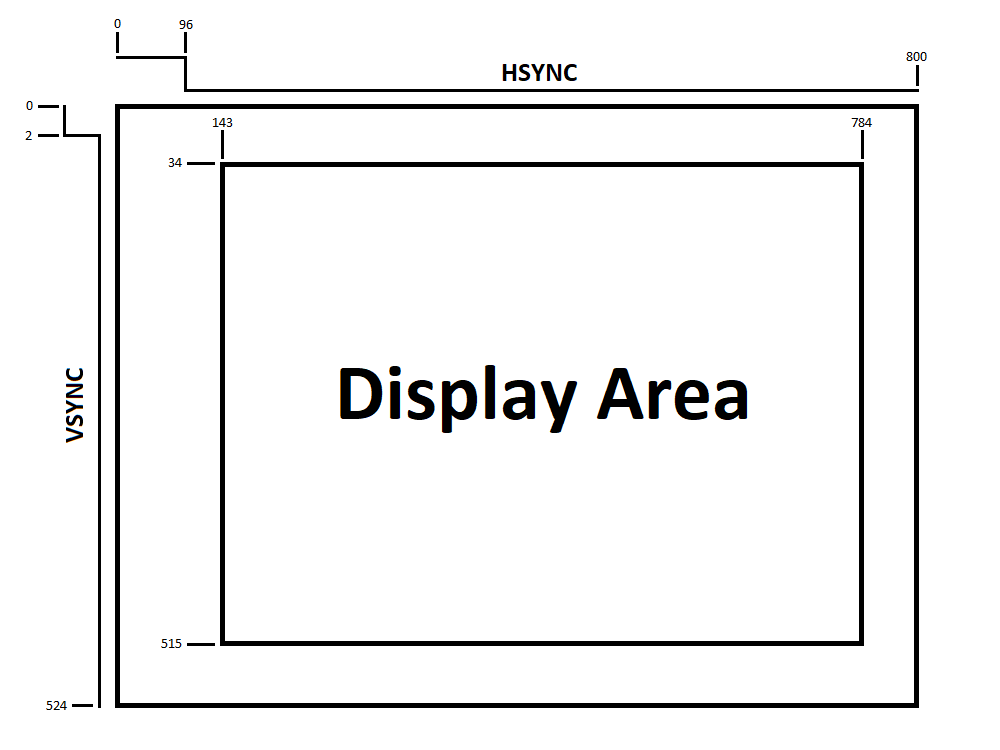
\includegraphics[scale=0.4]{vga.png}}
   \caption{Timing diagram for the VGA interface}
\end{figure} 
From the timing diagram, we can see that we need two counters namely a horizontal counter and a vertical counter.
To drive counters we need a clock with 25 MHz frequency. 
To obtain a clock signal with that frequency from the internal clock of the FPGA which has a 50 MHz frequency we implemented a clock divider circuit. 
After we obtained the clock signal with a 25 MHz frequency, we connected it to the horizontal counter. 
Horizontal counter counts at every clock cycle, and it counts from 0 to 800. Vertical counter counts 1 when the horizontal counter hits 800. 
We have two synchronization outputs namely HYSNC and VSYNC to tell the monitor beginning and ending of a row and frame respectively. 
HSYNC is high when the horizontal counter is between 0 and 96, and VSYNC is high when the vertical counter is between 0 and 2. 
Altera FPGA uses a digital-to-analog converter that takes 8-bit input for each color channel and converts it to an analog signal that has a voltage between 
0 and 5 Volts. \cite{fpga} \\
\par When the horizontal counter is between 143 and 784, and the vertical counter is between 34 and 515, RGB values of the pixel at the point (hcounter - 143, ycounter - 34) are returned to the DAC of the FPGA. 
We implemented a \textit{rgbSelector} module to get the RGB values for a given coordinate on the display. 
If the given coordinate is in the board region, the module finds the corresponding block coordinate and reads which piece is 
placed to that coordinate from the memory. Then it gets the RGB value from the memory module that corresponds to the piece. 
If the given coordinate is not in the board region but in a region that involves a text or picture, it reads the RGB value from the corresponding memory. 
If it is neither in the board region nor a picture or text region, then it returns a white color. \\
\par Since we need only 5 colors (white, black, red, green, and blue), we encoded and stored pictures that we used with 1 bit for each color channel. 
After the \textit{rgbSelector} module returns RGB values with 1 bit for each channel, 
another module we called \textit{vgaDecoder} converts it to output with 8 bits for each color channel and returns it to the DAC of the FPGA. \\
\par When the counters are not in the display area, 0 is returned to the DAC of the FPGA. 
An example of the display is shown in Figure 2, below.  
\begin{figure}[H]
  \centerline{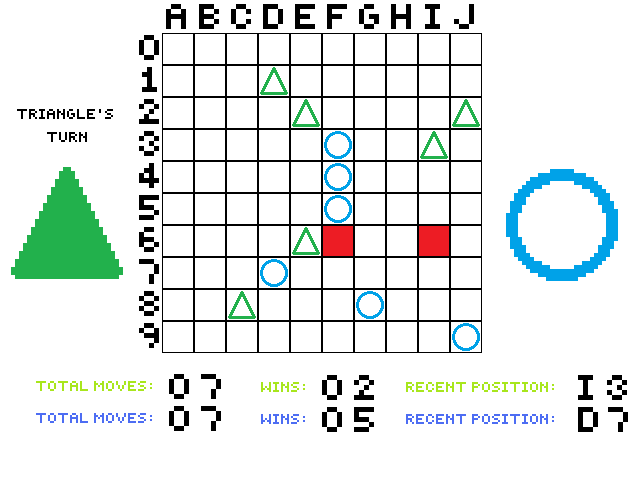
\includegraphics[scale=0.65, frame]{sample_board.png}}
   \caption{Example of the display}
\end{figure} 
\subsection{Button Debouncing and Edge Detector}
In this project, we need to get three inputs, \textbf{logic 1}, \textbf{logic 0}, and \textbf{activity}, from the user by using push buttons on the FPGA. However, due to mechanical and physical issues, pushbuttons often generate noisy signals called dirty bounces, and these bounces prevent us from properly triggering the program. Thus, to eliminate these undesirable effects, we used the \textit{debouncer\_delayed} module that makes a noisy pushbutton input signal to the ideal input case. \\
\par The working principle of the \textit{debouncer\_delayed} module is quite simple. When a button is pressed, the timer is going to count the elapsed time up to a predefined threshold parameter. If the timer hits the threshold value, the program concludes that the button has reached its steady state and has been pressed. Similarly, when the button is released and the steady state is reached, the program concludes that the button has been released. \\
\par After debouncing the button input, we designed another module called \textit{edge\_detector} to detect the negative and positive edges of the debounced input so that we will use the edge signals directly as button signals in the game controller. \\
\par The \textit{button} module contains both \textit{debouncer\_delayed} and \textit{edge\_detector} modules so that the hierarchical design principle is followed throughout the project. Also, both of these modules, are written like a state machine to make it easier to implement condition-based and flexible code. The waveform simulation result of the \textit{button} module in Quartus II is given in Figure 3. Besides these, in the \textit{button\_top} module each button is defined separately in a hierarchical manner by using the \textit{button} module.
 \begin{figure}[H]
   \centerline{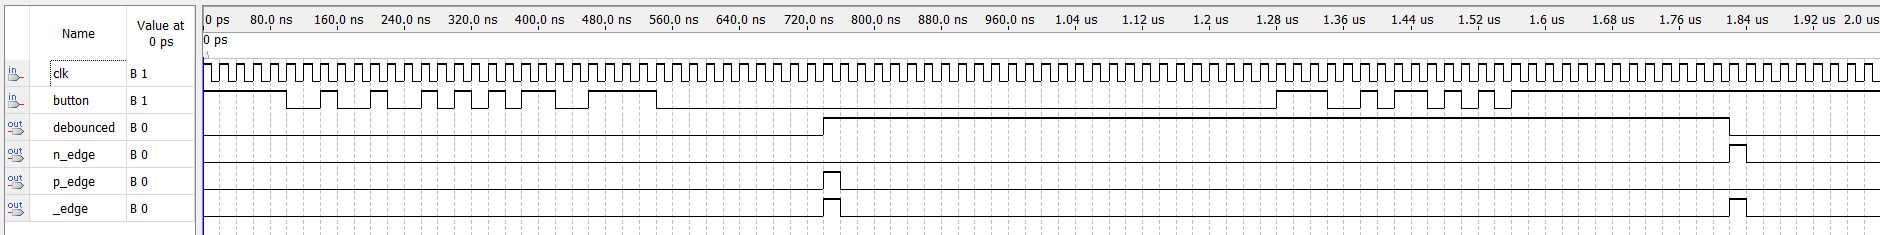
\includegraphics[scale=0.22]{simulation.png}}
    \caption{Button module, waveform simulation result}
\end{figure} 
\subsection{Game Engine}
As shown in Figure 4, the game engine can be modeled as a state machine that consists of 5 separate states: an input processing state (parse\_inp), an invalid move checking state (invld\_mv), a bookkeeping state, a state that checks if a win condition is satisfied, and finally, a state that resets the game board with appropriate modifications to the scores. Before discussing the states any further, it is helpful to understand the general encoding scheme of the board and shapes. \\
\subsubsection{Shape Encoding and Board Layout}
\par  The shapes are encoded using 2 bits as follows:
\begin{itemize}
  \item Empty (no shape): 00
  \item Triangle: 01
  \item Circle: 10
  \item Square: 11
\end{itemize}
\par Encoding the shapes in this way has several advantages. The first and most obvious is the ability to keep track of triangle and circle turns using a single variable -say currTurn- and if a player’s turn is over, the bits can simply be inverted to give the other player the ability to place their shape. The other advantages will be discussed in the relevant states in the report.
   \begin{figure}
   \centering \resizebox{8cm}{!}{
   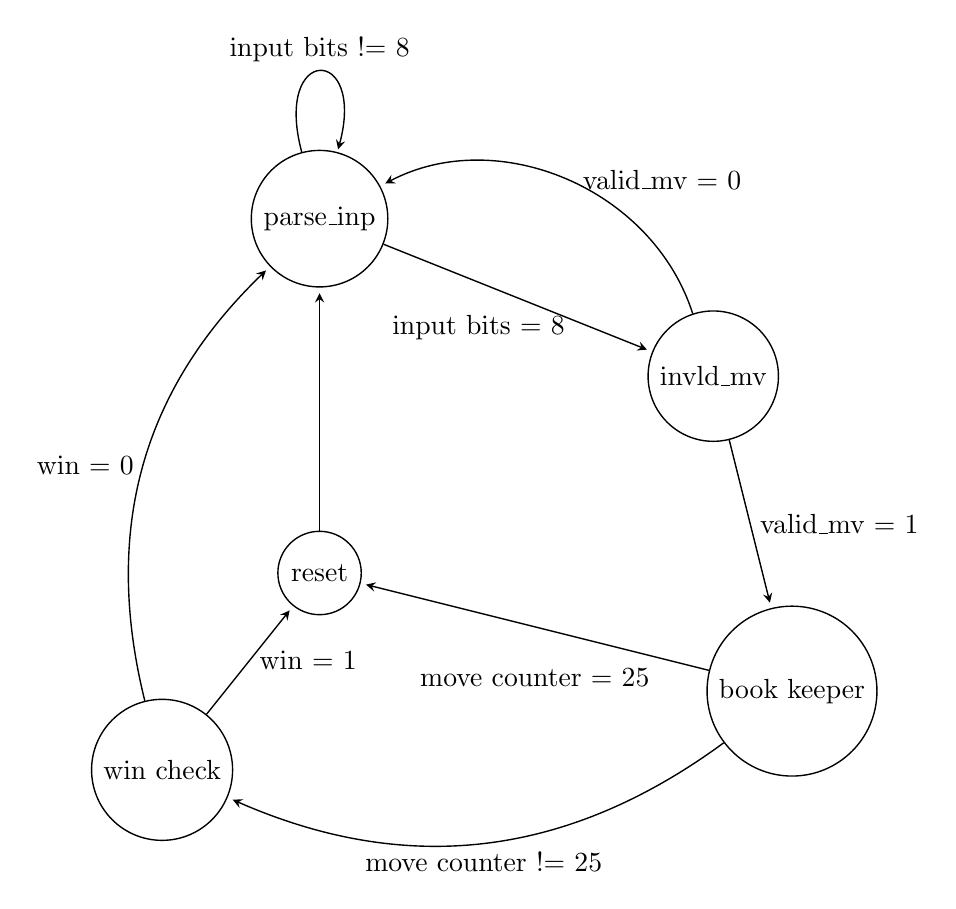
\begin{tikzpicture}[ - > , >= stealth, shorten >=2pt , line width =0.5 pt , node distance =2 cm]
   \node [circle , draw] (parse) at (0 , 0) {parse\_inp};
   \node [circle , draw] (invalid) at (5 , -2) {invld\_mv};
   \node [circle , draw] (book) at (6 , -6) {book keeper};
   \node [circle , draw] (reset) at (0 , -4.5) {reset};
   \node [circle , draw] (win) at (-2 , -7) {win check};
  
   \path (parse) edge [loop above] node [above] {input bits != 8} (parse) ;
   \path (invalid) edge [bend right=50] node [right, xshift=0.1cm] {valid\_mv = 0} (parse) ;
   \path (book) edge [bend left] node [below] {move counter != 25} (win) ;
   \path (win) edge [bend left] node [left] {win = 0} (parse) ;
   \path (win) edge node [right] {win = 1} (reset) ;
   \path (parse) edge node [below, xshift=-0.5cm, yshift=-0.1cm] {input bits = 8} (invalid) ;
   \path (book) edge node [below, yshift=-0.4cm] {move counter = 25} (reset) ;
   \path (invalid) edge node [right] {valid\_mv = 1} (book) ;
   \path (reset) edge node [above] {} (parse) ;
   \end{tikzpicture}}
   \caption{State machine of the game engine}
   \end{figure}
   \subsubsection{Input Parsing}
   The input parsing state has the sole role of converting the binary input into x and y coordinates. This is done through the use of two counters – one for the y and the other for x. The counters allow for easy inversion of the order of the input bits and for checking whether the used has provided 8 bits or not. \\
\subsubsection{Invalid Move Checking}
If the activity button is pressed after the user has provided 8 bits, the state machine moves on to invld\_mv. In this state two main checks are performed: \begin{itemize} 
\item The x and y coordinates specified by the user are within range, i.e., the coordinates are greater than or equal to zero and less than 10. This is done using simple if statements.
\item The specified coordinate is empty. This can be done by taking the OR operator of the two bits of the encoding scheme specified above. Only an empty cell will give zero, if the state is occupied the result of the operator will be one.
\end{itemize}
\subsubsection{Bookkeping}
The game board can be modeled as a 2-bit 100 cell wide memory block. A position is stored in the board as follows: \(y \cdot 10 + x\). In this encoding scheme, the y position is stored in the tens place while the x position is stored in the ones place. Furthermore, another array called bookkeeper is used to (as the name suggests) keep track of all player movements in sequential order. \\
\par Since the bookkeeper keeps track of movement coordinates sequentially, erasing every sixth move becomes just a trivial task of accessing the bookkeeper array at the appropriate index, using the info retrieved from that array to write 11 to the board. \\
\subsubsection{Win Checking Algorithm} 
A win condition can be only created after the last move that is placed on the board. That is why, instead of checking the whole board we just check the area around the last move. To do that we define several offsets: dx, dy, positive diagonal offset, and negative diagonal offset used to check rows, columns, diagonals with positive slopes, and finally diagonals with negative slopes respectively. The slopes are defined with respect to the coordinate system shown in Figure 5.
 \begin{figure}[H]
   \centerline{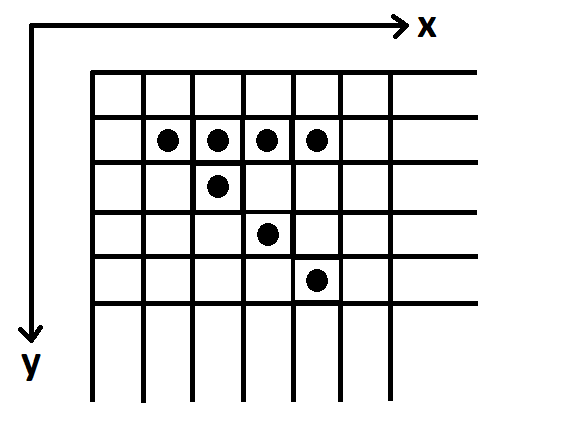
\includegraphics[scale=0.6]{check.png}}
    \caption{Button module, waveform simulation result}
\end{figure} 
The win checking state is itself a state machine with two distinct states: 
\begin{itemize}
\item Looping limit calculations
\item Consecutive shape counting
\end{itemize}
To understand the algorithm better consider Figure 5, above. \\
\paragraph{Consecutive Shape Counting}
To count consecutive shapes one can, add the previously defined offsets to the x and y coordinates and keep track of the similar shapes using a counter. Depending on the slope one can add the offsets as follows:
\begin{itemize}
\item Rows: \(y \cdot 10 + x + dx \)
\item Columns: \((y + dy) \cdot 10 + x\) 
\item Positive Diagonals: \((y + \text{diagoffset}) \cdot 10 + x + \text{diagoffset}\)
\item Negative Diagonals: \((y - \text{diagoffset}) \cdot 10 + x + \text{diagoffset}\)
\end{itemize} \hfill \hfill
\par Note that the offsets can be negative and that the offsets count from the minimum possible coordinate up to the maximum possible coordinate. Thus, an implementation detail that should not be forgotten is to reset the consecutive shape counter if the sequence is broken, otherwise the algorithm might give a false positive. \\
\paragraph{Row and Column Limit Calculations} The minimum possible limit for looping is -3 regardless of the slope type. However, this value cannot be hardcoded due to the edge cases. Consider what happens if the player selects the coordinate B1 as the last move (figure add figure number). Then the minimum offset that should be added to the row cannot exceed -1, otherwise the array index bounds will be exceeded. The same applies for the maximum offset. Thus the looping limits for row checking can be defined as follows: \begin{equation}\resizebox{0.9\hsize}{!}{$
\text{dxmin} =
\begin{cases}
 -3 &\text{ if x \(\geq\) D} \\ -x &\text{, otherwise} 
\end{cases} \qquad 
\text{dxmax} =
\begin{cases}
 3 &\text{ if x \(\leq\) G} \\ 10-x &\text{, otherwise} 
\end{cases}$}
\end{equation} \\
\paragraph{Positive and Negative Diagonal Limit Calculations}
There is a little more subtlety involved in calculating the diagonal looping limits due to the fact that both x and y coordinates should be taken into account. Again, consider input B1. In this case, the minimum offset is obviously  -1  = dxmin = dymin = posmin. Now let’s consider the input C1. In this case the minimum diagonal looping limit is bounded by the y coordinate since it is smaller. Thus, it can be concluded that the looping limits of the diagonals depend on the looping limits of rows and columns. The same logic can be repeated for several test cases to obtain the following formulas:
\begin{itemize}
\item Posdiagmin = min\{dxmin, dymin\}
\item Posdiagmax = min\{dxmax, dymax\}
\item Negdiagmin = min\{dxmax, dymin\}
\item Negdiagmax = min\{dxmin, dymax\}
\end{itemize} \hfill \hfill
\subsubsection{Resetting}
Resetting is triggered if either a draw or win condition is created. In either case the board game is wiped by writing 00 to all cells. The bookkeeper array is also wiped, and the appropriate counters are reset. The game state is set to parse input in preparation for a new game.
\section{Conclusion}

\bibliographystyle{ieeetr}
\bibliography{refs}
\end{document}
